\newpage
\section{CÁC SỐ ĐẶC TRƯNG ĐO XU THẾ TRUNG TÂM CỦA MẪU SỐ LIỆU}
\subsection{LÝ THUYẾT CẦN NHỚ}
\subsubsection{Số trung bình cộng (số trung bình)}
	\begin{enumerate}[\iconMT]
		\item \indam{Định nghĩa:}
		\begin{boxdn}
			\textit{Số trung bình cộng} $\overline{x}$ của mẫu $n$ số liệu $x_1$, $x_2$, $\ldots$, $x_n$ là $\overline{x}=\dfrac{x_1+x_2+\cdots+x_n}{n}$.
		\end{boxdn}
		\item \indam{Chú ý:}
		\begin{boxdn}
			Số trung bình cộng còn được tính theo công thức sau
			\begin{itemize}
				\item $\overline{x}=\dfrac{n_1 x_1+n_2 x_2+\cdots+n_k x_k}{n}$, trong đó $n_1$, $n_2$, $\ldots$, $n_k$ lần lượt là \textbf{tần số} của các số liệu $x_1$, $x_2$, $\ldots$, $x_k$ và $n=n_1+n_2+\ldots+n_k$ là \textbf{cỡ mẫu}.
				\item $\overline{x}=f_1 x_1+f_2 x_2+\cdots+f_k x_k$, trong đó $f_1=\dfrac{n_1}{n}$, $f_2=\dfrac{n_2}{n}$, $\ldots$, $f_k=\dfrac{n_k}{n}$ lần lượt là \textbf{tần số tương đối} (hay còn gọi là \textbf{tần suất}) của các số liệu $x_1$, $x_2$, $\ldots$, $x_k$.
			\end{itemize}
		\end{boxdn}
	\end{enumerate}
%=================
\subsubsection{Trung vị}
\begin{enumerate}[\iconMT]
	\item \indam{Định nghĩa:}
	Sắp thứ tự mẫu số liệu gồm $n$ số liệu thành một dãy không giảm (hoặc không tăng).
	\begin{boxdn}
		\begin{itemize}
			\item Nếu $n$ là số lẻ thì số liệu đứng ở vị trí thứ $\dfrac{n+1}{2}$ (số đứng chính giữa) gọi là \textit{trung vị}.
			\item Nếu $n$ là số chẵn thì số trung bình cộng của hai số liệu đứng ở vị trí thứ $\dfrac{n}{2}$ và $\dfrac{n}{2}+1$ gọi là \textit{trung vị}.
		\end{itemize}
		Trung vị kí hiệu là $M_{\mathrm{e}}$.
	\end{boxdn}
\end{enumerate}
%=================
\subsubsection{Tứ phân vị}
\begin{enumerate}[\iconMT]
	\item \indam{Định nghĩa:}
	Sắp thứ tự mẫu số liệu gồm $n$ số liệu thành một dãy không giảm.
	\begin{boxdn}
		\textit{Tứ phân vị} của mẫu số liệu trên là bộ ba giá trị: tứ phân vị thứ nhất $Q_1$, tứ phân vị thứ hai $Q_2$ và tứ phân vị thứ ba $Q_3$. Ba giá trị này chia mẫu số liệu thành bốn phần có số lượng phần tử bằng nhau.
		\begin{itemize}
			\item Tứ phân vị thứ hai $Q_2$ chính là số trung vị của mẫu.
			\item Tứ phân vị thứ nhất $Q_1$ là trung vị của nửa số liệu đã sắp xếp bên trái $Q_2$ (không bao gồm $Q_2$ nếu $n$ lẻ).
			\item Tứ phân vị thứ ba $Q_3$ là trung vị của nửa số liệu đã sắp xếp bên phải $Q_2$ (không bao gồm $Q_2$ nếu $n$ lẻ).
		\end{itemize}
	\end{boxdn}
\end{enumerate}
%=================
\subsubsection{Mốt}
\begin{enumerate}[\iconMT]
	\item \indam{Định nghĩa:}
	\begin{boxdn}
		\textit{Mốt} của mẫu số liệu là giá trị có tần số lớn nhất trong bảng phân bố tần số và kí hiệu là $M_o$.
	\end{boxdn}
	\item \indam{Chú ý:} Một mẫu số liệu có thể có một hoặc nhiều mốt.
\end{enumerate}
%-------------------------------------------------------------------------------------------
\subsection{PHÂN LOẠI VÀ PHƯƠNG PHÁP GIẢI TOÁN}
\begin{dang}{Xác định số trung bình cộng của mẫu số liệu}
	Dựa vào định nghĩa, ta có $\overline{x}=\dfrac{x_1+x_2+\cdots+x_n}{n}$.
\end{dang}
\begin{vd}%[0D6N3-2]%[Dự án D - Đề cương 3 khối 10-11-12 NH25-26 - Nguyễn Tiến]
	Bốn bạn Bình, Cường, Hoa, Kiên cùng thi vào trường phổ thông chất lượng cao Bình Minh. Kết quả thi được cho bởi bảng thống kê sau
	\begin{center}
		\begin{tabular}{|*{4}{>{\centering\arraybackslash}m{3cm}|}}
			\hline
			\textbf{Học sinh} & \textbf{Điểm Toán} & \textbf{Điểm Ngữ Văn} & \textbf{Điểm Tiếng Anh} \\
			\hline
			Bình & $10$ & $8$ & $9$ \\
			\hline
			Cường & $6$ & $7$ & $5$ \\
			\hline
			Hoa & $10$ & $10$ & $4$ \\
			\hline
			Kiên & $9$ & $5$ & $10$ \\
			\hline
		\end{tabular}
	\end{center}
	Tính điểm trung bình kết quả thi $3$ môn Toán, Ngữ Văn, Tiếng Anh của mỗi bạn và cho biết bạn nào trúng tuyển. Biết rằng, nếu muốn trúng tuyển, điểm trung bình các môn thi ở trên phải lớn hơn hoặc bằng $8$ và không môn nào dưới $5$ điểm.
	\loigiai{
		Điểm trung bình kết quả thi của các bạn Bình, Cường, Hoa, Kiên lần lượt là
		\allowdisplaybreaks
		\begin{eqnarray*}
			&\overline{x}_B=\dfrac{10+8+9}{3}=9; \qquad\qquad & \overline{x}_C=\dfrac{6+7+5}{3}=6;\\
			&\overline{x}_H=\dfrac{10+10+4}{3}=8; \qquad\qquad & \overline{x}_K=\dfrac{9+5+10}{3}=8.
		\end{eqnarray*}
		Dựa vào các số liệu trên, ta thấy bạn Bình và bạn Kiên trúng tuyển.
	}
\end{vd}
%=================
\begin{dang}{Xác định trung vị của mẫu số liệu}
	\begin{itemize}
		\item Sắp thứ tự mẫu số liệu gồm $n$ số liệu thành một dãy không giảm (hoặc không tăng).
		\item Nếu $n$ là số lẻ thì trung vị $M_{\mathrm{e}}$ bằng giá trị thứ $\dfrac{n+1}{2}$; nếu $n$ là số chẵn thì trung vị $M_{\mathrm{e}}$ bằng trung bình cộng của hai giá trị thứ $\dfrac{n}{2}$ và $\dfrac{n}{2}+1$.
	\end{itemize}
\end{dang}
\begin{vd}%[0D6N3-3]%[Dự án D - Đề cương 3 khối 10-11-12 NH25-26 - Nguyễn Tiến]
	Đầu năm học, nhà trường cho học sinh khám sức khỏe. Mẫu số liệu thống kê kết quả đo cân nặng (đơn vị: ki-lô-gam) của $7$ bạn nam đầu tiên như sau
	\begin{center}
		\begin{tabular}{*{7}{>{\centering\arraybackslash}m{1cm}}}
			$64$ & $58$ & $62{,}1$ & $55$ & $67$ & $61$ & $60{,}5$
		\end{tabular}
	\end{center}
	Trung vị của mẫu số liệu trên là bao nhiêu?
	\loigiai{
		Sắp xếp các số liệu của mẫu trên theo thứ tự không giảm
		\begin{center}
			\begin{tabular}{*{7}{>{\centering\arraybackslash}m{1cm}}}
				$55$ & $58$ & $60{,}5$ & $61$ & $62{,}1$ & $64$ & $67$
			\end{tabular}
		\end{center}
		Mẫu số liệu trên có $7$ số liệu và số liệu thứ tư là $61$.\\
		Vì vậy $M_{\mathrm{e}}=61$ (kg).
	}
\end{vd}
\begin{vd}%[0D6N3-3]%[Dự án D - Đề cương 3 khối 10-11-12 NH25-26 - Nguyễn Tiến]
	Mẫu số liệu thống kê chiều cao (đơn vị: xăng-ti-mét) của $10$ bạn tổ $I$ lớp $10A$ như sau
	\begin{center}
		\begin{tabular}{*{10}{>{\centering\arraybackslash}m{1cm}}}
			$164$ & $156$ & $170$ & $168$ & $158$ & $173$ & $167$ & $161$ & $157$ & $174$
		\end{tabular}
	\end{center}
	Trung vị của mẫu số liệu trên là bao nhiêu?
	\loigiai{
		Sắp xếp các số liệu của mẫu trên theo thứ tự không giảm
		\begin{center}
			\begin{tabular}{*{10}{>{\centering\arraybackslash}m{1cm}}}
				$156$ & $157$ & $158$ & $161$ & $164$ & $167$ & $168$ & $170$ & $173$ & $174$
			\end{tabular}
		\end{center}
		Mẫu số liệu trên có $10$ số liệu; số liệu thứ năm và thứ sáu lần lượt là $164$ và $167$.\\
		Vì vậy $M_{\mathrm{e}}=\dfrac{164+167}{2}=165{,}5$ (cm).
	}
\end{vd}
%=================
\begin{dang}{Xác định tứ phân vị của mẫu số liệu}
	Sắp thứ tự mẫu số liệu gồm $n$ số liệu thành một dãy không giảm. Khi đó
	\begin{itemize}
		\item Tứ phân vị thứ hai $Q_2$ chính là số trung vị của mẫu.
		\item Tứ phân vị thứ nhất $Q_1$ là trung vị của nửa số liệu đã sắp xếp bên trái $Q_2$ (không bao gồm $Q_2$ nếu $n$ lẻ).
		\item Tứ phân vị thứ ba $Q_3$ là trung vị của nửa số liệu đã sắp xếp bên phải $Q_2$ (không bao gồm $Q_2$ nếu $n$ lẻ).
	\end{itemize}
\end{dang}
\begin{vd}%[0D6N3-4]%[Dự án D - Đề cương 3 khối 10-11-12 NH25-26 - Nguyễn Tiến]
	Mẫu số liệu thống kê số cân nặng (đơn vị: ki-lô-gam) tăng thêm của $7$ trẻ sơ sinh trong ba tháng đầu tiên như sau
	\begin{center}
		\begin{tabular}{*{7}{>{\centering\arraybackslash}m{1cm}}}
			$0{,}9$ & $1{,}0$ & $1{,}1$ & $1{,}14$ & $1{,}18$ & $1{,}2$ & $1{,}3$
		\end{tabular}
	\end{center}
	Tứ phân vị của mẫu số liệu trên là bao nhiêu?
	\loigiai{
		Mẫu số liệu trên đã được sắp xếp theo thứ tự không giảm.\\
		Trung vị của mẫu số liệu trên là $1{,}14$.\\
		Trung vị của dãy số liệu $0{,}9$; $1{,}0$; $1{,}1$ là $1{,}0$.\\
		Trung vị của dãy số liệu $1{,}18$; $1{,}2$; $1{,}3$ là $1{,}2$.\\
		Vậy $Q_1=1{,}0$; $Q_2=1{,}14$; $Q_3=1{,}2$.
	}
\end{vd}
\begin{vd}%[0D6N3-4]%[Dự án D - Đề cương 3 khối 10-11-12 NH25-26 - Nguyễn Tiến]
	Mẫu số liệu thống kê thời gian (đơn vị: phút) đọc hết một cuốn sách của $9$ bạn tổ $I$ lớp $10A$ như sau
	\begin{center}
		\begin{tabular}{*{9}{>{\centering\arraybackslash}m{1cm}}}
			$102$ & $130$ & $118$ & $127$ & $115$ & $138$ & $121$ & $109$ & $132$
		\end{tabular}
	\end{center}
	Tứ phân vị của mẫu số liệu trên là bao nhiêu?
	\loigiai{
		Sắp xếp các số liệu của mẫu trên theo thứ tự không giảm
		\begin{center}
			\begin{tabular}{*{9}{>{\centering\arraybackslash}m{1cm}}}
				$102$ & $109$ & $115$ & $118$ & $121$ & $127$ & $130$ & $132$ & $138$
			\end{tabular}
		\end{center}
		Trung vị của mẫu số liệu trên là $121$.\\
		Trung vị của dãy số liệu $102$, $109$, $115$, $118$ là $\dfrac{109+115}{2}=112$.\\
		Trung vị của dãy số liệu $127$, $130$, $132$, $138$ là $\dfrac{130+132}{2}=131$.\\
		Vậy $Q_1=112$, $Q_2=121$, $Q_3=131$.
	}
\end{vd}
%=================
\begin{dang}{Xác định mốt của mẫu số liệu}
	\begin{itemize}
		\item Lập bảng phân bố tần số của mẫu số liệu.
		\item Mốt $M_o$ là giá trị có tần số lớn nhất trong bảng phân bố tần số.
	\end{itemize}
\end{dang}
\begin{vd}%[0D6H3-5]%[Dự án D - Đề cương 3 khối 10-11-12 NH25-26 - Nguyễn Tiến]
	Một cửa hàng bán giày thống kê số đôi giày bán được trong Quý $III$ năm $2020$ như sau
	\begin{center}
		\begin{tabular}{|>{\centering\arraybackslash}m{4cm}|*{8}{>{\centering\arraybackslash}m{0.75cm}|}}
			\hline
			\textbf{Cỡ giày} & \textbf{37} & \textbf{38} & \textbf{39} & \textbf{40} & \textbf{41} & \textbf{42} & \textbf{43} & \textbf{44} \\
			\hline
			Số đôi giày bán được
			\newline (Tần số) & $41$ & $49$ & $50$ & $71$ & $53$ & $46$ & $27$ & $5$ \\
			\hline
		\end{tabular}
	\end{center}
	\begin{enumerate}
		\item Mốt trong bảng tần số thống kê số giày bán ra trong Quý $III$ năm $2020$ của cửa hàng trên là bao nhiêu?
		\item Cửa hàng đó nên nhập về nhiều hơn cỡ giày nào để bán tiếp?
	\end{enumerate}
	\loigiai{
		\begin{enumerate}
			\item Vì tần số lớn nhất là $71$ và $71$ tương ứng với cỡ giày $40$ nên mốt của bảng trên là $40$.
			\item Cửa hàng nên nhập về nhiều hơn cỡ giày $40$ để bán tiếp vì số lượng giày cỡ $40$ bán được nhiều nhất.
		\end{enumerate}
	}
\end{vd}
%-------------------------------------------------------------------------------------------
\subsection{Bài tập rèn luyện}
\ind{PHẦN I.} \inden{Câu trắc nghiệm nhiều phương án lựa chọn. Mỗi câu hỏi học sinh chỉ chọn một phương án.}\\
\setcounter{ex}{0}
\Opensolutionfile{ans}[ans/0T6-Bai3-TN]%--Đặt tên 0T6-Bai3-Dang1-TN
\begin{ex}%[0D6N3-1]%[Dự án D - Đề cương 3 khối 10-11-12 NH25-26 - Nguyễn Tiến]%
	[\textit{Trích đề thi HKI - Trường THPT Chuyên Trần Phú, Hải Phòng - Năm học 2023-2024}]
	Các giá trị xuất hiện nhiều nhất trong mẫu số liệu được gọi là
	\choice
	{Số trung vị}
	{Số trung bình}
	{\True Mốt}
	{Cỡ mẫu}
	\loigiai{
		Các giá trị xuất hiện nhiều nhất trong mẫu số liệu được gọi là Mốt.
	}
\end{ex}
\begin{ex}%[0D6N3-1]%[Dự án D - Đề cương 3 khối 10-11-12 NH25-26 - Nguyễn Tiến]%
	[\textit{Trích đề thi HKI - Trường THPT Bùi Thị Xuân, TPHCM - Năm học 2023-2024}]
	Xác định cỡ mẫu của mẫu số liệu sau
	\begin{center}
		\begin{tabular}{*{11}{>{\centering\arraybackslash}m{0.5cm}}}
			$3$ & $7$ & $11$ & $5$ & $6$ & $8$ & $8$ & $9$ & $10$ & $15$ & $15$ \\
		\end{tabular} 
	\end{center}
	\choice
	{$10$}
	{$9$}
	{\True $11$}
	{$15$}
	\loigiai{
		Ta có cỡ mẫu $n=11$.
	}
\end{ex}
\begin{ex}%[0D6N3-1]%[Dự án D - Đề cương 3 khối 10-11-12 NH25-26 - Nguyễn Tiến]%
	[\textit{Trích đề thi HKI - Trường THPT Bùi Thị Xuân, TPHCM - Năm học 2023-2024}]
	Số điểm một cầu thủ bóng rổ ghi được trong $20$ trận đấu được cho bởi bảng sau:
	\begin{center}
		\begin{tabular}{|c|c|c|c|c|c|c|c|c|c|c|}
			\hline
			Điểm số	& $6$ & $8$ & $11$ & $14$ & $22$ & $25$ \\
			\hline
			Số trận & $1$ & $2$ & $5$ & $5$ & $3$ & $4$ \\
			\hline
		\end{tabular} 
	\end{center}
	Tần suất cầu thủ đó ghi được $8$ điểm là
	\choice
	{$\dfrac{2}{5}$}
	{$\dfrac{1}{5}$}
	{\True $\dfrac{1}{10}$}
	{$\dfrac{1}{4}$}
	\loigiai{
		Ta có cỡ mẫu số liệu là $n=1+2+5+5+3+4=20$.\\
		Tần suất cầu thủ đó ghi được $8$ điểm là $\dfrac{2}{20}=\dfrac{1}{10}$.
	}
\end{ex}
\begin{ex}%[0D6N3-2]%[Dự án D - Đề cương 3 khối 10-11-12 NH25-26 - Nguyễn Tiến]%
	[\textit{Trích đề thi HKI - Trường THPT Chuyên Hạ Long, Quảng Ninh - Năm học 2023-2024}]
	Cho mẫu số liệu
	\begin{center}
		\begin{tabular}{*{8}{>{\centering\arraybackslash}m{1cm}}}
			$23$ & $41$ & $71$ & $29$ & $48$ & $45$ & $72$ & $41$ \\
		\end{tabular}
	\end{center}
	Số trung bình của mẫu số liệu trên là
	\choice
	{\True $46{,}25$}
	{$47{,}36$}
	{$40{,}53$}
	{$43{,}89$}
	\loigiai{
		Ta có $\overline{x}=\dfrac{23+41+71+29+48+45+72+41}{8}=46{,}25$.
	}
\end{ex}
\begin{ex}%[0D6N3-2]%[Dự án D - Đề cương 3 khối 10-11-12 NH25-26 - Nguyễn Tiến]%
	[\textit{Trích đề thi HKI - Trường THPT Chuyên Hùng Vương, Phú Thọ - Năm học 2024-2025}]
	Mẫu số liệu sau cho biết số ghế trống tại một rạp chiếu phim trong $9$ ngày
	\begin{center}
		\begin{tabular}{*{9}{>{\centering\arraybackslash}m{1cm}}}
			$9$ & $8$ & $22$ & $20$ & $18$ & $15$ & $19$ & $13$ & $11$ \\
		\end{tabular}
	\end{center}
	Số ghế trống trung bình trong $9$ ngày của rạp chiếu phim trên là
	\choice
	{$22$}
	{$18$}
	{\True $15$}
	{$135$}
	\loigiai{ 
		Số ghế trống trung bình trong $9$ ngày của rạp chiếu phim trên là
		$$\overline{x} = \dfrac{9+8+22+20+18+15+19+13+11}{9} = \dfrac{135}{9} = 15.$$
	}
\end{ex}
\begin{ex}%[0D6N3-2]%[Dự án D - Đề cương 3 khối 10-11-12 NH25-26 - Nguyễn Tiến]%
	[\textit{Trích đề thi HKI - Trường THPT Chuyên Hùng Vương, Phú Thọ - Năm học 2024-2025}]
	Cho bảng số liệu điểm kiểm tra môn Toán của $30$ học sinh như sau
	\begin{center}
		\begin{tabular}{|>{\centering\arraybackslash}m{2.5cm}|*{8}{>{\centering\arraybackslash}m{1cm}|}}
			\hline
			Điểm & $4$ & $5$ & $6$ & $7$ & $8$ & $9$ & $10$ & Cộng\\
			\hline
			Số học sinh & $1$ & $4$ & $6$ & $4$ & $9$ & $4$ & $2$ & $30$\\
			\hline
		\end{tabular}
	\end{center}
	Số trung bình của bảng số liệu trên là
	\choice
	{$7$}
	{$8$}
	{$7{,}5$}
	{\True $7{,}2$}
	\loigiai{
		Số trung bình cộng của bảng số liệu trên bằng
		$$\dfrac{4 \cdot 1 + 5 \cdot 4 +6 \cdot 6 +7 \cdot 4 +8 \cdot 9 + 9 \cdot 4 + 10 \cdot 2}{30}=7{,}2.$$
	}
\end{ex}
\begin{ex}%[0D6N3-2]%[Dự án D - Đề cương 3 khối 10-11-12 NH25-26 - Nguyễn Tiến]%
	[\textit{Trích đề thi HKI - Trường THPT Lê Thánh Tôn, TPHCM - Năm học 2023-2024}]
	Bảng số liệu sau cho biết thời gian chạy cự ly ngắn của các bạn lớp $10A$ (đơn vị giây) như sau
	\begin{center}
		\begin{tabular}{|>{\centering\arraybackslash}m{3cm}|*{6}{>{\centering\arraybackslash}m{1cm}|}}
			\hline
			Thời gian (giây) & $15$ & $16$ & $17$ & $18$ & $19$ & $20$ \\
			\hline
			Số bạn  & $5$ & $12$ & $6$ & $10$ & $5$ & $2$ \\
			\hline
		\end{tabular} 
	\end{center}
	Hãy tính thời gian chạy trung bình của các bạn.
	\choice
	{$16{,}5$}
	{$16$}
	{$17{,}5$}
	{\True $17{,}1$}
	\loigiai{
		Thời gian chạy trung bình của các bạn là
		$$\dfrac{5\cdot15+12\cdot16+6\cdot17+10\cdot18+5\cdot19+2\cdot20}{5+12+6+10+5+2}=17{,}1.$$
	}
\end{ex}
\begin{ex}%[0D6N3-2]%[Dự án D - Đề cương 3 khối 10-11-12 NH25-26 - Nguyễn Tiến]%
	[\textit{Trích đề thi HKI - Trường THPT Bùi Thị Xuân, TPHCM - Năm học 2023-2024}]
	Mẫu số liệu sau cho biết điểm số bài kiểm tra của các học sinh lớp $10$A
	\begin{center}
		\begin{tabular}{|c|c|}
			\hline
			Điểm & Số học sinh \\
			\hline
			$10$ & $8$ \\
			\hline
			$9$	& $7$ \\
			\hline
			$8$	&  $15$ \\
			\hline
			$7$	& $5$ \\
			\hline
			$6$	& $3$ \\
			\hline
			$5$	&  $2$ \\
			\hline
		\end{tabular}
	\end{center}
	Hãy tính điểm trung bình của điểm số bài kiểm tra của các học sinh lớp $10$A.
	\choice
	{\True $8{,}15$}
	{$8{,}5$}
	{$8{,}45$}
	{$8{,}55$}
	\loigiai{
		Điểm trung bình số điểm bài kiểm tra là
		$$\overline{x}=\dfrac{10\cdot 8+9\cdot 7+ 8\cdot 15+ 7\cdot 5+ 6\cdot 3+ 5\cdot 2}{8+7+15+5+3+2}=\dfrac{163}{20}=8{,}15.$$
	}
\end{ex}
\begin{ex}%[0D6N3-3]%[Dự án D - Đề cương 3 khối 10-11-12 NH25-26 - Nguyễn Tiến]%
	[\textit{Trích đề thi HKI - Trường THPT Bùi Thị Xuân, TPHCM - Năm học 2023-2024}]
	Mẫu số liệu sau thống kê số sách mỗi bạn học sinh Tổ $1$ đã đọc ở thư viện trường trong tháng $9$
	\begin{center}
		\begin{tabular}{*{9}{>{\centering\arraybackslash}m{1cm}}}
			$1$ & $1$ & $2$ & $3$ & $4$ & $4$ & $5$ & $6$ & $7$ \\
		\end{tabular}
	\end{center}
	Hãy xác định trung vị của mẫu số liệu trên.
	\choice
	{$1$}
	{$3$}
	{$7$}
	{\True $4$}
	\loigiai{
		Cỡ mẫu $n=9$ nên trung vị mẫu số liệu là $M_{\mathrm{e}}=4$.
	}
\end{ex}
\begin{ex}%[0D6N3-3]%[Dự án D - Đề cương 3 khối 10-11-12 NH25-26 - Nguyễn Tiến]%
	[\textit{Trích đề thi HKI - Trường THPT Tân Túc, TPHCM - Năm học 2023-2024}]
	Trung vị của mẫu số liệu $4$; $5$; $8$; $13$; $5$; $17$; $9$ là
	\choice
	{$9$}
	{$5$}
	{$13$}
	{\True $8$}
	\loigiai{
		Sắp xếp mẫu số liệu thành dãy không giảm $4$; $5$; $5$; $8$; $9$; $13$; $17$.\\
		Trung vị của mẫu số liệu là $M_{\mathrm{e}}=8$.	
	}
\end{ex}
\begin{ex}%[0D6N3-3]%[Dự án D - Đề cương 3 khối 10-11-12 NH25-26 - Nguyễn Tiến]%
	[\textit{Trích đề thi HKI - Trường THPT Bùi Thị Xuân, TPHCM - Năm học 2023-2024}]
	Mẫu số liệu sau thống kê số xe đạp đã bán được trong năm $2022$ của của hàng A là
	\begin{center}
		\begin{tabular}{*{12}{>{\centering\arraybackslash}m{0.5cm}}}
			$10$ & $7$ & $8$ & $3$ & $7$ & $15$ & $25$ & $16$ & $17$ & $9$ & $8$ & $7$ \\
		\end{tabular}
	\end{center}
	Hãy xác định trung vị của mẫu số liệu trên.
	\choice
	{$7$}
	{$8$}
	{$20$}
	{\True $8{,}5$}
	\loigiai{
		Sắp xếp mẫu số liệu thành dãy không giảm, ta được
		\begin{center}
			\begin{tabular}{*{12}{>{\centering\arraybackslash}m{0.5cm}}}
				$3$ & $7$ & $7$ & $7$ & $8$ & $8$ & $9$ & $10$ & $15$ & $16$ & $17$ & $25$ \\
			\end{tabular}
		\end{center}
		Do cỡ mẫu của mẫu số liệu trên bằng $12$ nên trung vị của mẫu số liệu là $\dfrac{8+9}{2}=8{,}5$.
	}
\end{ex}
\begin{ex}%[0D6N3-4]%[Dự án D - Đề cương 3 khối 10-11-12 NH25-26 - Nguyễn Tiến]%
	[\textit{Trích đề thi HKI - Trường THPT Chuyên Hạ Long, Quảng Ninh - Năm học 2023-2024}]
	Cho mẫu số liệu sau
	\begin{center}
		\begin{tabular}{*{11}{>{\centering\arraybackslash}m{0.7cm}}}
			$156$ & $156$ & $157$ & $158$ & $159$ & $160$ & $161$ & $161$ & $161$ & $162$ & $164$ \\
		\end{tabular}
	\end{center}
	Tứ phân vị thứ nhất của mẫu số liệu trên là
	\choice
	{\True $157$}
	{$158$}
	{$159$}
	{$156$}
	\loigiai{
		Ta có mẫu số liệu đã được sắp xếp theo thứ tự không giảm và cỡ mẫu là $11$.\\
		Suy ra tứ phân vị thứ nhất chính là trung vị của phần số liệu gồm $156$; $156$; $157$; $158$; $159$.\\
		Vậy $Q_{1}=157$.
	}
\end{ex}
\begin{ex}%[0D6N3-4]%[Dự án D - Đề cương 3 khối 10-11-12 NH25-26 - Nguyễn Tiến]%
	[\textit{Trích đề thi HKI - Trường THPT Tân Túc, TPHCM - Năm học 2023-2024}]
	Số lượng ly trà sữa một quán nước bán được trong 1 tuần qua là
	\begin{center}
		\begin{tabular}{*{7}{>{\centering\arraybackslash}m{1cm}}}
			$9$ & $25$ & $13$ & $25$ & $30$ & $11$ & $36$ \\
		\end{tabular}
	\end{center}
	Tứ phân vị thứ ba của mẫu số liệu trên là
	\choice
	{$11$}
	{\True $30$}
	{$36$}
	{$25$}
	\loigiai{
		Ta viết lại mẫu số liệu trên thành dãy không giảm như sau
		\begin{center}
			\begin{tabular}{*{7}{>{\centering\arraybackslash}m{1cm}}}
				$9$ & $11$ & $13$ & $25$ & $25$ & $30$ & $36$ \\
			\end{tabular}
		\end{center}
		Giá trị của tứ phân vị thứ ba $Q_3$ chính là trung vị của phần số liệu $25$; $30$; $36$ nên $Q_3=30$.
	}
\end{ex}
\begin{ex}%[0D6N3-5]%[Dự án D - Đề cương 3 khối 10-11-12 NH25-26 - Nguyễn Tiến]%
	[\textit{Trích đề thi HKI - Trường THPT Tân Túc, TPHCM - Năm học 2023-2024}]
	Một cửa hàng giày thể thao đã thống kê cỡ giày của một số khách hàng nữ được chọn ngẫu nhiên
	\begin{center}
		\begin{tabular}{|>{\centering\arraybackslash}m{2.5cm}|*{5}{>{\centering\arraybackslash}m{1cm}|}}
			\hline Cỡ giày & $35$ & $36$ & $37$ & $38$ & $39$ \\
			\hline Số lượng & $4$ & $8$ & $13$ & $2$ & $1$ \\
			\hline
		\end{tabular}
	\end{center}
	Cửa hàng nên nhập cỡ giày nào với số lượng nhiều nhất?
	\choice
	{\True $37$}
	{$35$}
	{$36$}
	{$38$}
	\loigiai{
		Cỡ giày $37$ có số lượng khách nhiều nhất do đó cửa hàng nên nhập cỡ giày $37$ nhiều nhất.	
	}
\end{ex}
\begin{ex}%[0D6N3-5]%[Dự án D - Đề cương 3 khối 10-11-12 NH25-26 - Nguyễn Tiến]%
	[\textit{Trích đề thi HKI - Trường THPT Hoàng Việt, DakLak - Năm học 2023-2024}]
	Số lượng laptop của một cửa hàng bán được trong quý II năm $2021$ được cho bởi bảng dưới đây.
	\begin{center}
		\begin{tabular}{|>{\centering\arraybackslash}m{3.3cm}|*{6}{>{\centering\arraybackslash}m{1.2cm}|}}
			\hline Hãng & Dell & HP & Lenovo & Apple & Razer & Asus \\
			\hline Số laptop bán được & $60$ & $55$ & $45$ & $30$ & $15$ & $42$ \\
			\hline
		\end{tabular}
	\end{center}
	Mốt của bảng số liệu trên là
	\choice
	{\True Dell}
	{HP}
	{Apple}
	{Lenovo}
	\loigiai{
		Mốt của bảng số liệu trên là Dell (vì có tần số lớn nhất).
	}
\end{ex}
\begin{ex}%[0D6H3-2]%[Dự án D - Đề cương 3 khối 10-11-12 NH25-26 - Nguyễn Tiến]%
	[\textit{Trích đề thi HKI - Trường THPT Chuyên Hùng Vương, Phú Thọ - Năm học 2023-2024}]
	Theo Báo cáo kính tế - xã hội năm $2022$ của Tổng cục Thống kê về Tổng GDP tính bằng USD của Việt Nam từ năm $2015$ đến hết năm $2022$ được cho dưới dạng biểu đồ sau
	\begin{center}
		Biểu đồ. \textbf{Tổng GDP tính bằng USD theo tỷ giá hối đoái}.\quad Đơn vị: tỷ USD
		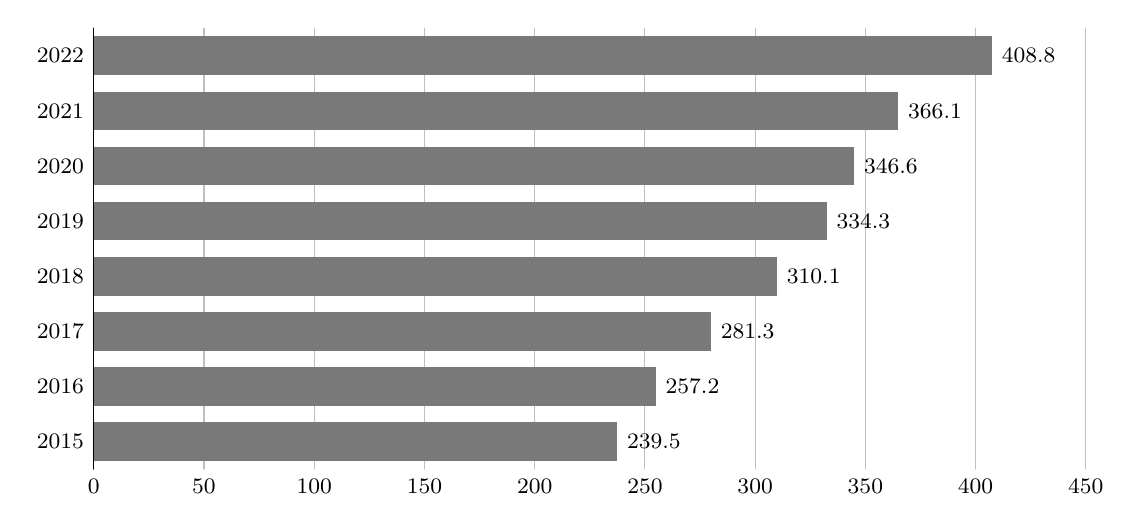
\begin{tikzpicture}[scale=0.7, font=\footnotesize, line join=round, line cap=round, >=stealth]
			\def\h{0.7}
			%				\fill[red!93!black] (-1.7,9-0.5*\h) rectangle (-1.2,9+0.5*\h);
			%				\fill[gray!50] (-1.4,9-0.5*\h) rectangle (18.3,9+0.5*\h);
			%				\node at (-1.5,9)[right]{Biểu đồ. \textbf{Tổng GDP tính bằng USD theo tỷ giá hối đoái}};
			%				\node at (18.3,9)[left]{Đơn vị: tỷ USD};
			\foreach \x in {0,50,...,450}{
				\draw[gray!50] (\x/25,8.5)--(\x/25,0.5) node[below]{\color{black}$\x$};
			}
			\foreach \nam/\GDP in {2015/239.5,2016/257.2,2017/281.3,2018/310.1,2019/334.3,2020/346.6,2021/366.1,2022/408.8}{
				\pgfmathsetmacro{\x}{int(\GDP/2.5)/10};
				\pgfmathsetmacro{\y}{int(\nam-2014)};
				\fill[gray!95!black] (0,\y-0.5*\h) rectangle (\x,\y+0.5*\h);
				\node at (0,\y)[left]{\color{black}$\nam$};
				\node at (\x,\y)[right]{\color{black}$\GDP$};
			}
			\draw (0,8.5)--(0,0.5);
		\end{tikzpicture}
	\end{center}
	Bình quân tổng GDP tính bằng USD từ năm $2015$ đến hết năm $2022$ của Việt Nam bằng
	\choice
	{$317{,}8$}
	{$318{,}2$}
	{\True $318$}
	{$317{,}9$}
	\loigiai{
		Ta có trung bình GDP là
		$$\overline{x}=\dfrac{239,5+257,2+281,3+310,1+334,3+346,6+366,1+408,8}{8}\approx 318.$$
	}
\end{ex}
\begin{ex}%[0D6H3-3]%[Dự án D - Đề cương 3 khối 10-11-12 NH25-26 - Nguyễn Tiến]%
	[\textit{Trích đề thi HKI - Trường THPT Lê Thánh Tôn, TPHCM - Năm học 2023-2024}]
	Cho bảng số liệu thống kê điểm của $47$ học sinh trong một bài kiểm tra thường xuyên môn toán như sau
	\begin{center}
		\begin{tabular}{|>{\centering\arraybackslash}m{2.5cm}|*{8}{>{\centering\arraybackslash}m{0.5cm}|}}
			\hline
			Điểm & $3$ & $4$ & $5$ & $6$ & $7$ & $8$ & $9$ & $10$ \\
			\hline
			Số học sinh & $1$ & $3$ & $6$ & $9$ & $10$ & $12$ & $4$ & $2$ \\
			\hline
		\end{tabular}
	\end{center}
	Tìm trung vị của mẫu số liệu trên.
	\choice
	{\True $7$}
	{$7{,}5$}
	{$8{,}5$}
	{$6$}
	\loigiai{
		Số giá trị của mẫu số liệu trên là $n=1+3+6+9+10+12+4+2=47$.\\
		Trung vị của mẫu số liệu trên là giá trị thứ $\dfrac{n+1}{2}=\dfrac{47+1}{2}=24$ là $M_{\mathrm{e}}=7$.
	}
\end{ex}
\begin{ex}%[0D6H3-4]%[Dự án D - Đề cương 3 khối 10-11-12 NH25-26 - Nguyễn Tiến]%
	[\textit{Trích đề thi HKI - Trường THPT Phan Bội Châu, Bình Thuận - Năm học 2023-2024}]
	Cho mẫu số liệu: $9$; $\,9$; $\,10$; $\,8$; $\,9$; $\,10$; $\, 10$; $\,7$; $\,8$; $\,8$; $\,10$; $\,9$; $\,8$. Tứ phân vị thứ $3$ của mẫu số liệu trên là
	\choice
	{$8$}
	{$9$}
	{$7$}
	{\True $10$}
	\loigiai{
		Sắp xếp mẫu số liệu theo thứ tự không giảm là 
		$$7;\quad 8;\quad 8;\quad 8;\quad 8;\quad 9;\quad 9;\quad 9;\quad 9;\quad 10;\quad 10;\quad 10;\quad 10.$$
		Vì mẫu số liệu có 13 phần tử là số lẻ nên số trung vị của mẫu số là $Q_2=9$.\\
		Tứ phân vị thứ 3  là trung vị của nửa số liệu bên phải là $Q_3=\dfrac{10+10}{2}=10$.
	}
\end{ex}
\begin{ex}%[0D6H3-5]%[Dự án D - Đề cương 3 khối 10-11-12 NH25-26 - Nguyễn Tiến]%
	[\textit{Trích đề thi HKI - Trường THPT Bùi Thị Xuân, TPHCM - Năm học 2023-2024}]
	Mẫu số liệu sau cho biết mức lương của các nhận viên trong một công ty (đơn vị: triệu đồng)
	\begin{center}
		\begin{tabular}{*{9}{>{\centering\arraybackslash}m{1cm}}}
			$8$ & $6$ & $15$ & $6$ & $12$ & $10$ & $8$ & $7$ & $6$ \\
		\end{tabular}
	\end{center}
	Hãy xác định mốt của mức lương các nhân viên của công ty trên.
	\choice
	{$12$}
	{\True $6$}
	{$15$}
	{$8$}
	\loigiai{
		Bảng tần số cho mẫu số liệu trên là
		\begin{center}
			\begin{tabular}{|>{\centering\arraybackslash}m{2.5cm}|*{6}{>{\centering\arraybackslash}m{1cm}|}}
				\hline
				Mức lương & $6$ & $7$ & $8$ & $10$ & $12$ & $15$\\
				\hline
				Số nhân viên & $3$ & $1$ & $2$ & $1$ & $1$ & $1$\\
				\hline
			\end{tabular}
		\end{center}
		Số liệu có tần số lớn nhất là $6$.\\
		Vậy mốt của mẫu số liệu trên là $6$ (triệu đồng).
	}
\end{ex}
\begin{ex}%[0D6H3-5]%[Dự án D - Đề cương 3 khối 10-11-12 NH25-26 - Nguyễn Tiến]%
	[\textit{Trích đề thi HKI - Trường THPT Bùi Thị Xuân, TPHCM - Năm học 2023-2024}]
	Thống kê số sản phẩm các công nhân ở tổ làm được trong một ngày được ghi lại ở bảng sau
	\begin{center}
		\begin{tabular}{*{10}{>{\centering\arraybackslash}m{1cm}}}
			$16$ & $12$ & $18$ & $13$ & $14$ & $15$ & $16$ & $17$& $12$ & $13$
		\end{tabular} 
	\end{center}
	Mẫu số liệu trên có bao nhiêu mốt?
	\choice
	{$2$}
	{\True $3$}
	{$1$}
	{$0$}
	\loigiai{
		Bảng tần số cho mẫu số liệu trên là
		\begin{center}
			\begin{tabular}{|>{\centering\arraybackslash}m{2.5cm}|*{7}{>{\centering\arraybackslash}m{1cm}|}}
				\hline
				Số sản phẩm	& $12$ & $13$ & $14$ & $15$ & $16$ & $17$ &$18$\\
				\hline
				Tần số & $2$ & $2$ & $1$ & $1$ & $2$ & $1$ &$1$\\
				\hline
			\end{tabular} 
		\end{center}
		Tần số xuất hiện nhiều nhất trong mẫu số liệu là $2$.\\
		Nên mẫu số liệu đã cho có ba mốt là $12$, $13$ và $16$.
	}
\end{ex}
\Closesolutionfile{ans}
%=================
\ind{PHẦN II.} \inden{Câu trắc nghiệm đúng sai. Trong mỗi ý a), b), c), d) ở mỗi câu, học sinh chọn đúng hoặc sai.}\\
\setcounter{ex}{0}
\Opensolutionfile{ans}[ans/0T6-Bai3-DS]%--Đặt tên 0T6-Bai3-DS
\begin{ex}%[0D6H3-1]%[Dự án D - Đề cương 3 khối 10-11-12 NH25-26 - Nguyễn Tiến]%
	[\textit{Trích đề thi HKI - Trường THPT Chuyên Hùng Vương, Phú Thọ - Năm học 2023-2024}]
	Xét tính đúng, sai của các khẳng định sau
	\choiceTF
	{\True Tứ phân vị thứ ba không nhỏ hơn tứ phân vị thứ nhất}
	{Trung vị luôn bằng giá trị trung bình của mẫu số liệu}
	{Trong mẫu số liệu có $30\%$ số liệu nhỏ hơn hoặc bằng tứ phân vị thứ nhất}
	{Mốt là tần số lớn nhất của mẫu số liệu}
	\loigiai{
		\begin{itemchoice}
			\itemch Tứ phân vị thứ ba không nhỏ hơn tứ phân vị thứ nhất.
			\itemch Trung vị khác với giá trị trung bình của mẫu số liệu.
			\itemch Vì có $25\%$ số liệu nhỏ hơn hoặc bằng tứ phân vị thứ nhất.
			\itemch Mốt là giá trị có tần số lớn nhất.
		\end{itemchoice}
	}
\end{ex}
\begin{ex}%[0D6H3-4]%[Dự án D - Đề cương 3 khối 10-11-12 NH25-26 - Nguyễn Tiến]%
	[\textit{Trích đề thi HKI - Trường THPT Nguyễn Chí Thanh, Lâm Đồng - Năm học 2023-2024}]
	Bảng sau đây cho biết chiều cao của một nhóm học sinh
	\begin{center}
		\begin{tabular}{cccccccc}
			$160$ & $178$ & $150$ & $164$ & $168$ & $176$ & $156$ & $172$ \\
		\end{tabular}
	\end{center}
	\choiceTF
	{Tứ phân vị thứ hai lớn hơn số trung vị của mẫu số liệu}
	{Tứ phân vị thứ nhất bằng $166$}
	{\True Tứ phân vị thứ ba là một số chia hết cho $3$}
	{\True $Q_1+Q_3=2\cdot Q_2$}
	\loigiai{
		Sắp xếp mẫu số liệu theo thứ tự không giảm
		$$\begin{array}{llllllll} $150$ & $156$ & $160$ & $164$ & $168$ & $172$ & $176$ & $178$ \end{array}$$
		Vì cỡ mẫu là $8$ là số chẵn nên giá trị tứ phân vị thứ hai là $Q_2=\dfrac{x_4+x_5}{2}=\dfrac{164+168}{2}=166$.\\
		Tứ phân vị thứ nhất là trung vị của mẫu: $150$; $156$; $160$; $164$.\\
		Do đó $Q_1=\dfrac{x_2+x_3}{2}=\dfrac{156+160}{2}=158$.\\
		Tứ phân vị thứ ba là trung vị của mẫu: $168$; $172$; $176$; $178$.\\
		Do đó $Q_3=\dfrac{x_6+x_7}{2}=\dfrac{172+176}{2}=174$.\\
		\begin{itemchoice}
			\itemch Tứ phân vị thứ hai chính là số trung vị của mẫu số liệu.
			\itemch Tứ phân vị thứ nhất là $Q_1=158$.
			\itemch Tứ phân vị thứ ba là $Q_3=174$ là số chia hết cho $3$.
			\itemch Ta có $Q_1+Q_3=332=2\cdot 166$ nên $Q_1+Q_3=2\cdot Q_2$.
		\end{itemchoice}
	}
\end{ex}
\begin{ex}%[0D6H3-5]%[Dự án D - Đề cương 3 khối 10-11-12 NH25-26 - Nguyễn Tiến]
	Cho mẫu số liệu thống kê về sản lượng chè thu được trong $1$ năm (kg/sào) của $10$ hộ gia đình
	\begin{center}
		\begin{tabular}{|*{10}{>{\centering\arraybackslash}m{1cm}|}}
			\hline
			$112$ & $111$ & $112$ & $113$ & $114$  & $116$ & $115$ & $114$ & $115$ & $114$ \\
			\hline
		\end{tabular}
	\end{center}
	Khi đó
	\choiceTF
	{\True Sản lượng chè trung bình thu được trong một năm của mỗi gia đình là $113{,}6$ (kg/sào)}
	{Ta viết lại mẫu số liệu trên theo thứ tự không giảm là: $116$; $115$; $115$; $114$; $114$; $114$; $113$; $112$; $112$; $111$}
	{Số trung vị là $113$}
	{\True $114$ là mốt của mẫu số liệu đã cho}
	\loigiai{
		\begin{itemchoice}
			\itemch Sản lượng chè trung bình thu được trong một năm của mỗi gia đình là
			$$\overline{x}=\dfrac{112+111+112+113+114+116+115+114+115+114}{10}=113{,}6.$$
			\itemch Ta viết lại mẫu số liệu trên theo thứ tự không giảm
			\begin{center}
				\begin{tabular}{*{10}{c}}
					$111$ & $112$ & $112$ & $113$ & $114$  & $114$ & $114$ & $115$ & $115$ & $116$ \\
				\end{tabular}
			\end{center}
			\itemch Số giá trị của mẫu là $n=10$ (chẵn) nên trung bình cộng hai số chính giữa mẫu chính là trung vị.\\
			Vậy số trung vị là $\dfrac{114+114}{2}=114$.
			\itemch Trong mẫu trên, giá trị $114$ xuất hiện nhiều nhất ($3$ lần) nên $114$ là mốt của mẫu số liệu đã cho.
		\end{itemchoice}
	}
\end{ex}
\begin{ex}%[0D6V3-5]%[Dự án D - Đề cương 3 khối 10-11-12 NH25-26 - Nguyễn Tiến]%
	[\textit{Trích đề thi HKI - Trường THPT Chuyên Hùng Vương, Phú Thọ - Năm học 2024-2025}]
	Kết quả kiểm tra cuối kì I môn Toán (thang điểm $10$) của hai lớp $10A$ và $10B$ được thống kê như sau
	\begin{figure}[htb]
		\begin{minipage}{0.48\textwidth}
			\centering
			% Code cho hình vẽ thứ nhất
			\begin{tabular}{|c|c|c|c|c|}
				\hline $2$ & $7$ & $6$ & $3$ & $9$\\
				\hline $8$ & $6$ & $7$ & $9$ & $2$\\
				\hline $5$ & $7$ & $5$ & $9$ & $8$\\
				\hline $8$ & $7$ & $4$ & $3$ & $5$\\
				\hline $5$ & $4$ & $5$ & $7$ & $7$\\
				\hline
			\end{tabular}\\
			\text{Lớp 10A}
		\end{minipage}
		\hfill
		\begin{minipage}{0.48\textwidth}
			\centering
			% Code cho hình vẽ thứ hai
			\begin{tabular}{|c|c|c|c|c|}
				\hline $6$ & $7$ & $6$ & $4$ & $7$\\
				\hline $9$ & $3$ & $8$ & $7$ & $5$\\
				\hline $5$ & $6$ & $8$ & $7$ & $4$\\
				\hline $5$ & $3$ & $10$ & $7$ & $9$\\
				\hline $6$ & $7$ & $6$ & $7$ & $5$\\
				\hline
			\end{tabular}\\
			\text{Lớp 10B}
		\end{minipage}
	\end{figure}
	\choiceTF
	{\True Trung vị của mẫu số liệu ở lớp $10B$ là $6$}
	{\True Điểm trung bình môn Toán của lớp $10A$ là $5{,}92$}
	{\True Điểm trung bình môn Toán của lớp $10B$ là $6{,}28$}
	{Mốt của mẫu số liệu ở lớp $10A$ nhỏ hơn mốt của mẫu số liệu ở lớp $10B$}
	\loigiai{
		\begin{itemchoice}
			\itemch Sắp xếp các giá trị của số liệu theo thứ tự không giảm ở lớp $10B$ ta được mẫu số liệu sau
			$$3 \quad 3 \quad 4 \quad 4 \quad 5 \quad 5 \quad 5 \quad 5 \quad 6 \quad 6 \quad 6 \quad 6 \quad 6 \quad 7 \quad 7 \quad 7 \quad 7 \quad 7 \quad 7 \quad 7 \quad 8 \quad 8 \quad 9 \quad 9 \quad 10 \quad$$
			Mẫu số liệu có $25$ giá trị nên trung vị của mẫu là giá trị thứ $13$.\\
			Vậy trung vị $M_e=6$.
			\itemch Điểm trung bình môn Toán của lớp $10A$ là\\
			$$\overline{x}=\dfrac{2 \cdot 2+2 \cdot 3+ 2 \cdot 4+ 5 \cdot 5+ 2 \cdot 6 + 6 \cdot 7 + 3 \cdot 8+ 3 \cdot 9}{25}=5{,}92.$$
			\itemch Điểm trung bình môn Toán của lớp $10B$ là\\
			$$\overline{x}=\dfrac{2 \cdot 3+ 2 \cdot 4+ 4 \cdot 5+ 5 \cdot 6 + 7 \cdot 7 + 2\cdot 8+ 2 \cdot 9+1\cdot 10}{25}=6{,}28.$$
			\itemch Mốt của mẫu số liệu ở cả hai lớp đều là $7$.
		\end{itemchoice}
	}
\end{ex}
\begin{ex}%[0D6V3-5]%[Dự án D - Đề cương 3 khối 10-11-12 NH25-26 - Nguyễn Tiến]%
	[\textit{Trích đề thi HKI - Trường THPT Bình Phú, TPHCM - Năm học 2023-2024}]
	Số bàn thắng ghi được ở mỗi trận đấu của đội bóng đá $A$ trong một mùa giải được thống kê như sau
	\begin{center}
		\begin{tabular}{|*{7}{c|}}
			\hline
			Số bàn thắng & $0$ & $1$ & $2$ & $3$ & $4$ & $6$ \\
			\hline
			Số trận & $5$ & $10$ & $6$ & $5$ & $3$ & $1$ \\
			\hline
		\end{tabular}
	\end{center}
	\choiceTF
	{Ở bất kì trận đấu nào, đội bóng $A$ cũng đều có bàn thắng}
	{\True Số bàn thắng trung bình mà đội bóng đá $A$ ghi được trong một trận đấu của mùa giải là khoảng $1{,}83$}
	{Mốt của mẫu số liệu đã cho là $10$}
	{\True Số trung vị của mẫu số liệu đã cho là $1{,}5$}
	\loigiai{
		\begin{itemchoice}
			\itemch Có $5$ trận đấu mà đội bóng $A$ không ghi được bàn thắng nào.
			\itemch Ta có tổng số trận đấu là $30$ trận đấu.\\
			Ta có
			$\overline{x} = \dfrac{0\cdot 5 + 1\cdot 10 + 2\cdot 6 + 3\cdot 5 + 4\cdot 3 + 6\cdot 1}{30} = \dfrac{11}{6} \approx 1{,}83$.\\
			Vậy số bàn thắng trung bình mà đội bóng $A$ ghi được trong một trận đấu là khoảng $1{,}83$.
			\itemch Ta có mốt của mẫu số liệu là $1$.
			\itemch Sắp xếp mẫu số liệu theo thứ tự không giảm ta được $x_1 = 0$; $x_2= 0$; $\ldots$; $x_{30}= 6$.\\
			Do có $30$ giá trị nên $M_{\mathrm{e}} = \dfrac{1}{2} \left(x_{15} + x_{16}\right) = \dfrac{1}{2} (1 + 2) = 1{,}5$.
		\end{itemchoice}
	}
\end{ex}
\Closesolutionfile{ans}
%=================
\ind{PHẦN III.} \inden{Câu trả lời ngắn.}\\
\setcounter{ex}{0}
\Opensolutionfile{ans}[ans/0T6-Bai3-DS]%--Đặt tên 0T6-Bai3-DS
\begin{ex}%[0D6V3-2]%[Dự án D - Đề cương 3 khối 10-11-12 NH25-26 - Nguyễn Tiến]%
	[\textit{Trích đề thi HKI - Trường THPT Chuyên Hùng Vương, Phú Thọ - Năm học 2024-2025}]
	Tại một lớp học chứng chỉ Tin học, nếu điểm trung bình $5$ bài kiểm tra của học viên lớn hơn hoặc bằng $85$ điểm thì học viên sẽ được giảm $30 \%$ học phí. An đã làm $4$ bài kiểm tra với kết quả (điểm số) lần lượt là $94$; $82$; $78$; $80$. Hỏi bài cuối cùng An cần đạt được ít nhất bao nhiêu điểm để được giảm $30 \%$ học phí?
	\shortans[oly]{91}
	\loigiai{
		Giả sử bài kiểm tra cuối cùng An đạt được là $x$ (điểm) (điều kiện $x\geq 0$).\\
		Khi đó, điểm trung bình $5$ bài kiểm tra của An là 
		\begin{eqnarray*}
			& & \dfrac{94+82+78+80+x}{5}\geq 85\\
			&\Leftrightarrow & x+334\geq 425 \Leftrightarrow x\geq 91.
		\end{eqnarray*}
		Vậy bài cuối cùng của An cần đạt được ít nhất $91$ điểm để được giảm $30\%$ học phí.
	}
\end{ex}	
\begin{ex}%[0D6V3-2]%[Dự án D - Đề cương 3 khối 10-11-12 NH25-26 - Nguyễn Tiến]%
	[\textit{Trích đề thi HKI - Trường THPT Chuyên Huỳnh Mẫn Đạt, Kiên Giang - Năm học 2023-2024}]
	Sản lượng lúa (tạ) của $40$ thửa ruộng thí nghiệm có cùng diện tích được trình bày trong bảng phân bố tần số sau đây
	\begin{center}
		\begin{tabular}{|c|c|c|c|c|c|}
			\hline Sản lượng & $21$ & $22$ & $23$ & $24$ & $25$ \\
			\hline Tần số & $n$ & $8$ & $11$ & $10$ & $m$ \\
			\hline
		\end{tabular}
	\end{center}
	Biết rằng sản lượng lúa trung bình của $40$ thửa ruộng là $23{,}1$ tạ, khi đó $2n+3m$ bằng bao nhiêu?
	\shortans[oly]{28}
	\loigiai{
		Số trung bình của mẫu số liệu trên là 
		$$\overline{x}=\dfrac{21\cdot n+22\cdot 8+23\cdot11+24\cdot 10+25\cdot m}{40}.$$
		Theo đề bài ta có
		\allowdisplaybreaks
		\begin{eqnarray*}
			\overline{x}=23{,}1 &\Leftrightarrow & \dfrac{21\cdot n+22\cdot 8+23\cdot11+24\cdot 10+25\cdot m}{40}=23{,}1\\
			&\Leftrightarrow & 21n+25m=255.
		\end{eqnarray*}
		Lại có $n+8+11+10+m=40\Leftrightarrow m+n=11$.\\
		Do đó, ta có hệ phương trình $\heva{& 21n+25m=255 \\& m+n=11} \Leftrightarrow \heva{& m=6\\& n=5.}$\\
		Vậy $2n+3m=28$.
	}
\end{ex}
\begin{ex}%[0D6V3-5]%[Dự án D - Đề cương 3 khối 10-11-12 NH25-26 - Nguyễn Tiến]%
	[\textit{Trích đề thi HKI - Trường THPT Quang Trung, Hải Dương - Năm học 2023-2024}]
	Cho bảng phân bố tần số như sau
	\begin{center}
		\begin{tabular}{|>{\centering\arraybackslash}m{1.5cm}|*{8}{>{\centering\arraybackslash}m{1cm}|}}
			\hline Giá trị & $x_1$ & $x_2$ & $x_3$ & $x_4$ & $x_5$ & $x_6$ & $x_7$ & $x_8$ \\
			\hline Tần số & $15$ & $9 n-1$ & 12 & $n^2+7$ & 14 & 10 & $9 n-20$ & 17 \\
			\hline
		\end{tabular}
	\end{center}
	Tìm $n$ để các giá trị $M_0=x_2$ và $M_0=x_4$ là hai mốt của bảng số liệu trên.
	\shortans[oly]{8}
	\loigiai{
		Để các giá trị $M_0=x_2$ và $M_0=x_4$ là hai mốt của bảng số liệu thì điều kiện cần là
		$$9n-1=n^2+7  \Leftrightarrow n^2-9n+8=0 \Leftrightarrow \hoac{& n=1\\& n=8.}$$
		Với $n=1$ ta có tần số của $x_7$ là $n_7=9\cdot 1-20=-11 <0$ nên $n=1$ không thỏa.\\
		Với $n=8$ ta thấy thỏa đề bài.
	}
\end{ex}
\begin{ex}%[0D6V3-4]%[Dự án D - Đề cương 3 khối 10-11-12 NH25-26 - Nguyễn Tiến]%
	[\textit{Trích đề thi HKI - Trường THPT Hùng Vương, TPHCM - Năm học 2023-2024}]
	Chỉ số $IQ$ của một nhóm học sinh được thống kê trong bảng dữ liệu sau
	\begin{center}
		\begin{tabular}{cccccccccccc}
			$76$ & $83$ & $98$ & $85$ & $89$ & $96$ & $110$ & $98$ & $95$ & $78$ & $86$ & $95$ \\
		\end{tabular}
	\end{center}
	Tổng các tứ phân vị của mẫu số liệu trên là bao nhiêu?
	\shortans[oly]{273}
	\loigiai{
		Sắp xếp mẫu số liệu ta được dãy
		\begin{center}
			\begin{tabular}{cccccccccccc}
				$76$ & $78$ & $83$ & $85$ & $86$ & $89$ & $95$ & $95$ & $96$ & $98$ & $98$ & $110$ \\
			\end{tabular}
		\end{center}
		Vì cỡ mẫu bằng $12$, là số chẵn nên giá trị tứ phân vị thứ hai là 
		$$Q_2=\dfrac{1}{2}(89+95)=92.$$	
		Tứ phân vị thứ nhất là trung vị của mẫu 
		$$\begin{array}{llllll} 76 & 78 & 83 & 85 & 86 & 89 \end{array}$$
		Do đó $Q_1=\dfrac{1}{2}(83+85)=84$.\\
		Tứ phân vị thứ ba là trung vị của mẫu 
		$$\begin{array}{llllll} 95 & 95 & 96 & 98 & 98 & 110 \end{array}$$
		Do đó $Q_3=\dfrac{1}{2}(96+98)=97$.\\
		Vậy tổng các tứ phân vị của mẫu số liệu đã cho là
		$$Q_1+Q_2+Q_3=84+92+97=273.$$
	}
\end{ex}
\begin{ex}%[0D6V3-2]%[Dự án D - Đề cương 3 khối 10-11-12 NH25-26 - Nguyễn Tiến]%
	[\textit{Trích đề thi HKI - Trường THPT chuyên Lê Hồng Phong, TPHCM - Năm học 2023-2024}]
	Một học sinh lớp $10$ đã thực hiện một số bài kiểm tra môn Toán. Nếu bài kiểm tra tiếp theo em đạt được $10$ điểm thì điểm trung bình của em sẽ tăng lên $0{,}75$ điểm so với hiện nay. Nếu hai bài kiểm tra tiếp theo nữa (tổng cộng thêm ba bài) em đạt được $10$ điểm thì điểm trung bình của em sẽ tăng lên $1{,}5$ điểm so với hiện nay. Tìm điểm trung bình hiện nay của học sinh.
	\shortans[oly]{7}
	\loigiai{
		Gọi điểm trung bình hiện nay là $x$, số bài đã kiểm tra là $n$ ($0 \le x \le 10$, $n \in \mathbb{N^*}$).\\
		Điểm trung bình sau khi có thêm một bài kiểm tra đạt $10$ điểm là $\dfrac{nx+10}{n+1}$.\\
		Điểm trung bình sau khi có thêm ba bài kiểm tra đạt $10$ điểm là $\dfrac{nx+3\cdot 10}{n+3}$.\\
		Theo đề bài ta có hệ phương trình:\\
		\[\left\{\begin{aligned} &\dfrac{nx+10}{n+1} -x=0{,}75  \\ 
			&\dfrac{nx+3\cdot 10}{n+3} -x=1{,}5 \end{aligned}\right. 
		\Leftrightarrow \left\{\begin{aligned} &x+0{,}75n=9{,}25  \\ 
			&3x+ 1{,}5n=25{,}5 \end{aligned}\right. 
		\Leftrightarrow \left\{\begin{aligned} &x=7  \\ 
			&n=3. \end{aligned}\right. \]
		Vậy điểm trung bình ban đầu là $7$.
	}
\end{ex}
\Closesolutionfile{ans}
%=================
\ind{PHẦN IV.} \inden{Tự luận.}\\
\setcounter{ex}{0}
\begin{ex}%[0D6H3-2]%[Dự án D - Đề cương 3 khối 10-11-12 NH25-26 - Nguyễn Tiến]%
	[\textit{Trích đề thi HKI - Trường THPT Nguyễn Chí Thanh, TPHCM - Năm học 2023-2024}]
	Kết quả điểm thi học kì $1$ của một học sinh lớp $10$ như sau
	\begin{center}
		\begin{tabular}{|l|l|l|l|l|l|l|l|l|}
			\hline 4 & 9 &5 & 8 & 10 & 7 & 6 & 5 & 8 \\
			\hline
		\end{tabular}
	\end{center}
	Hãy tìm số trung bình của mẫu số liệu trên (làm tròn đến hàng phần trăm).
	\loigiai{
		Sắp xếp lại dãy số theo thứ tự không giảm$\colon 4;\quad 5;\quad 5;\quad 6;\quad 7;\quad 8;\quad 8;\quad 9;\quad 10$.\\
		Số trung bình cộng $\overline{x}=\dfrac{4+5\cdot 2+6+7+8\cdot 2+9+10}{9}\approx 6{,}89$.
	}
\end{ex}
\begin{ex}%[0D6H3-3]%[Dự án D - Đề cương 3 khối 10-11-12 NH25-26 - Nguyễn Tiến]%
	[\textit{Trích đề thi HKI - Trường THPT Nguyễn Thị Minh Khai, TPHCM - Năm học 2023-2024}]
	Điểm bài kiểm tra môn Toán trước khi thi học kỳ $I$ của lớp $10A1$ được cho dưới bảng sau
	\begin{center}
		\begin{tabular}{|c|c|c|c|c|c|c|c|}
			\hline \textbf{Điểm}        & $4$ & $5$ & $6$ & $7$  & $8$ & $9$ & $10$ \\
			\hline \textbf{Số học sinh} & $3$ & $5$ & $7$ & $12$ & $6$ & $8$ & $2$  \\
			\hline
		\end{tabular}
	\end{center}
	Để đánh giá mức độ học tập và có kế hoạch ôn thi phù hợp cho lớp, em hãy tính số trung bình và số trung vị của mẫu số liệu trên (Làm tròn kết quả đến $2$ chữ số sau dấu phẩy).
	\loigiai{
		Tổng số học sinh $n = 3 + 5 + 7 + 12 + 6 + 8 + 2 = 43$.
		\begin{itemize}
			\item Số trung bình là $\overline{x} = \dfrac{3 \cdot 4 + 5 \cdot 5 + 7 \cdot 6 + 12 \cdot 7 + 6 \cdot 8 + 8 \cdot 9 + 2 \cdot 10}{43} = \dfrac{303}{43} \approx 7{,}05$.
			\item Do $n = 43$ là số lẻ nên số trung vị của mẫu số liệu là học sinh thứ $22$. \\
			Vậy số trung vị của mẫu số liệu là $M_{\mathrm{e}} = 7$.
		\end{itemize}
	}
\end{ex}
\begin{ex}%[0D6N3-4]%[Dự án D - Đề cương 3 khối 10-11-12 NH25-26 - Nguyễn Tiến]%
	[\textit{Trích đề thi HKI - Trường THPT Chuyên Huỳnh Mẫn Đạt, Kiên Giang - Năm học 2023-2024}]
	Kết quả bài kiểm tra môn toán của một nhóm học sinh được ghi lại như sau
	$$
	\begin{array}{lllllllllllll}
		8 & 6 & 9 & 10 & 5 & 7 & 9 & 8 & 7 & 6 & 8 & 8 & 10
	\end{array}
	$$
	Tìm các tứ phân vị của mẫu số liệu trên.
	\loigiai{
		Sắp xếp lại mẫu số liệu theo thứ tự không giảm, ta được
		$$
		\begin{array}{lllllllllllll}
			5 & 6 & 6 & 7 & 7 & 8 & 8 & 8 & 8 & 9 & 9 & 10 & 10
		\end{array}
		$$
		Vì cỡ mẫu là $n=13$ là số lẻ nên
		\begin{itemize}
			\item Tứ phân vị thứ hai là $Q_2=8$.
			\item Tứ phân vị thứ nhất là $Q_1= 3{,}5$.
			\item Tứ phân vị thứ ba là $Q_3=10$.
		\end{itemize}
	}
\end{ex}
\begin{ex}%[0D6H3-4]%[Dự án D - Đề cương 3 khối 10-11-12 NH25-26 - Nguyễn Tiến]%
	[\textit{Trích đề thi HKI - Trường THPT Chuyên Lê Quý Đôn, Bình Định - Năm học 2023-2024}]
	Thống kê kết quả tham gia kì thi học sinh giỏi toán (thang điểm $20$) của $12$ học sinh như sau
	\begin{center}
		\begin{tabular}{*{12}{>{\centering\arraybackslash}m{0.75cm}}}
			$17$ & $17$ & $14$ & $14$ & $13$ & $13$ & $12$ & $19$ & $18$ & $16$ & $15$ & $15$ \\
		\end{tabular}
	\end{center}
	Tính số trung bình và các tứ phân vị của mẫu số liệu trên.
	\loigiai{
		Ta sắp xếp mấu số liệu trên theo thứ tự không giảm
		\begin{center}
			\begin{tabular}{*{12}{>{\centering\arraybackslash}m{0.75cm}}}
				$12$ & $13$ & $13$ & $14$ & $14$ & $15$ & $15$ & $16$ & $17$ & $17$ & $18$ & $19$ \\
			\end{tabular}
		\end{center}
		\begin{itemize}
			\item Số trung bình là $\overline{x}=\dfrac{12+13\cdot2+14\cdot2+15\cdot2+16+17\cdot2+18+19}{12}=15{,}25$.
			\item Vì $n=12$ nên tứ phân vị thứ hai là $Q_2=\dfrac{15+15}{2}=15$.
			\item Nửa số liệu bên trái $Q_2$ là $12 \quad 13 \quad 13 \quad 14 \quad 14 \quad 15$.\\
			Suy ra tứ phân vị thứ nhất là $Q_1=\dfrac{13+14}{2}=13{,}5$.
			\item Nửa số liệu bên phải $Q_2$ là $15 \quad 16 \quad 17\quad 17 \quad 18 \quad 19$ .\\
			Suy ra tứ phân vị thứ ba là $Q_3=\dfrac{17+17}{2}=17$.\\
			Vậy $Q_1=13{,}5$; $Q_2=15$; $Q_3=17$.
		\end{itemize}
	}
\end{ex}
\begin{ex}%[0D6H3-4]%[Dự án D - Đề cương 3 khối 10-11-12 NH25-26 - Nguyễn Tiến]%
	[\textit{Trích đề thi HKI - Trường THPT Hoàng Việt, DakLak - Năm học 2023-2024}]
	Thống kê cân nặng (đơn vị $\mathrm{kg}$ ) của $10$ trẻ sơ sinh ở một bệnh viện như sau
	\begin{center}
		\begin{tabular}{cccccccccc}
			$2{,}8$ & $3{,}2$ & $3{,}3$ & $2{,}6$ & $3{,}0$ & $2{,}5$ & $3{,}0$ & $2{,}8$ & $3{,}5$ & $3{,}3$ \\
		\end{tabular}
	\end{center}
	\begin{enumerate}
		\item  Tính số trung bình của mẫu số liệu trên.
		\item  Xác định các tứ phân vị của mẫu số liệu trên.
	\end{enumerate}
	\loigiai{
		\begin{enumerate}
			\item Số trung bình của mẫu số liệu là
			$$
			\overline{x}=\dfrac{2{,}8+3{,}2+3{,}3+2{,}6+3{,}0+2{,}5+3{,}0+2{,}8+3{,}5+3{,}3}{10}=3{,}0.
			$$
			\item Sắp xếp mẫu số liệu theo thứ tự không giảm, ta được
			$$
			\begin{array}{llllllllll}
				2{,}5 & 2{,}6 & 2{,}8 & 2{,}8 & 3{,}0 & 3{,}0 & 3{,}2 & 3{,}3 & 3{,}3 & 3{,}5.
			\end{array}
			$$
			Ta có $Q_2=\dfrac{3{,}0+3{,}0}{2}=3{,}0$.\\
			Từ đó suy ra $Q_1=2{,}8$ và $Q_3=3{,}3$.
		\end{enumerate}
	}
\end{ex}
\begin{ex}%[0D6H3-4]%[Dự án D - Đề cương 3 khối 10-11-12 NH25-26 - Nguyễn Tiến]%
	[\textit{Trích đề thi HKI - Trường THPT Như Văn Lan, Hải Phòng - Năm học 2023-2024}]
	Mẫu số liệu sau đây cho biết số lượng trường Trung học phổ thông ở Đồng bằng sông Cửu Long 
	\begin{center}
		$\begin{array}{lllllllllllll}
			33&34&33&29&24&39&42&24&23&19&24&15&26.
		\end{array}$
	\end{center}
	\begin{enumerate}[a)]
		\item Tính số trung bình.
		\item Tìm các tứ phân vị.
	\end{enumerate}
	\loigiai{
		\begin{enumerate}[a)]
			\item Số trung bình của mẫu số liệu
			$$\overline{x}=\dfrac{33+34+33+29+24+39+42+24+23+19+24+15+26}{13} \approx 28{,}08.$$
			\item Sắp xếp số liệu trên theo thứ tự không giảm ta được
			\begin{center}
				$\begin{array}{lllllllllllll}
					15&19&23&24&24&24&26&29&33&33&34&39&42.
				\end{array}$
			\end{center}
			\begin{itemize}
				\item Tứ phân vị thứ hai là $Q_2=26$.
				\item Tứ phân vị thứ nhất là $Q_1=\dfrac{23+24}{2}=23{,}5$.
				\item Tứ phân vị thứ ba là $Q_3=\dfrac{33+34}{2}=33{,}5$.
			\end{itemize}
		\end{enumerate}
	}
\end{ex}
\begin{ex}%[0D6H3-5]%[Dự án D - Đề cương 3 khối 10-11-12 NH25-26 - Nguyễn Tiến]%
	[\textit{Trích đề thi HKI - Trường THPT Trần Quang Khải, TPHCM - Năm học 2023-2024}]
	Khối lượng cơ thể trưởng thành của $10$ con chim  được ghi lại ở bảng sau (đơn vị: gram)
	\begin{center}
		\begin{tabular}{cccccccccc}
			$155$ & $165$ & $150$ & $155$ & $165$ & $170$ & $165$ & $150$ & $155$ & $160$ \\
		\end{tabular}
	\end{center}	
	Em hãy lập bảng tần số, tính khối lượng trung bình và mốt của mẫu số liệu trên.
	\loigiai{
		Bảng tần số của mẫu số liệu là
		\begin{center}
			\begin{tabular}{|c|c|c|c|c|c|}
				\hline
				Khối lượng(gram) & $150$ & $155$ & $160$ & $165$ & $170$ \\	\hline
				Số lượng (con) & $2$ & $3$ & $1$ & $3$ & $1$ \\ \hline
			\end{tabular}
		\end{center}
		Khối lượng trung bình của mẫu số liệu là
		$$\overline{x}=\dfrac{150\cdot 2+155\cdot 3+160\cdot 1+165\cdot 3+170\cdot 1}{10}=159\ \text{gram}.$$
		Mốt của dãy số liệu là $155$ và $165$.	
	}
\end{ex}
\begin{ex}%[0D6V3-3]%[Dự án D - Đề cương 3 khối 10-11-12 NH25-26 - Nguyễn Tiến]%
	[\textit{Trích đề thi HKI - Trường THPT Hồ Thị Bi, TPHCM - Năm học 2023-2024}]
	Cân nặng của $12$ vận động viên môn bơi lội của một câu lạc bô được ghi lại ở bảng sau:
	\begin{center}
		\begin{tabular}{|*{6}{>{\centering\arraybackslash}m{1.5cm}|}}
			\hline
			$51$ & $54$ & $51$ & $57$& $60$ & $59$\\
			\hline
			$60$ & $59$ & $52$ & $57$ & $52$ & $51$\\
			\hline 
		\end{tabular}
	\end{center}
	\begin{enumerate}
		\item Lập bảng tần số cho mẫu số liệu trên.
		\item Tính số trung bình, trung vị của mẫu số liệu trên.
	\end{enumerate}
	\loigiai{
		\begin{enumerate}
			\item Bảng tần số cho mẫu số liệu trên.
			\begin{center}
				\begin{tabular}{|>{\centering\arraybackslash}m{1.5cm}|*{6}{>{\centering\arraybackslash}m{1cm}|}}
					\hline
					Giá trị & $51$ & $52$ & $54$ & $57$ & $59$ & $60$ \\
					\hline
					Tần số & $3$ & $2$ & $1$ & $2$ & $2$ & $2$  \\
					\hline  
				\end{tabular} 
			\end{center}
			\item Số cân nặng trung bình của $12$ động viên là
			$$\dfrac{51 \cdot 3 + 52 \cdot 2 + 54 + 57 \cdot 2 + 59 \cdot 2 + 60 \cdot 2}{12} \approx 55{,}25.$$
			Trung vị $M_e=\dfrac{54+57}{2}=55{,}5$.
		\end{enumerate}
	}
\end{ex}
\begin{ex}%[0D6V3-5]%[Dự án D - Đề cương 3 khối 10-11-12 NH25-26 - Nguyễn Tiến]%
	[\textit{Trích đề thi HKI - Trường THPT Võ Thị Sáu, TPHCM - Năm học 2023-2024}]
	Khối lượng cơ thể lúc trưởng thành của $10$ con chim được ghi lại ở bảng sau (đơn vị: gam)
	\begin{center}
		\begin{tabular}{*{10}{>{\centering\arraybackslash}p{0.8cm}}}
			$155$ & $165$ & $150$ & $155$ & $165$ & $170$ & $165$ & $150$ & $155$ & $160$ \\
		\end{tabular}
	\end{center}
	Hãy tìm số trung bình, các tứ phân vị và mốt của mẫu số liệu trên.
	\loigiai{
		Sắp xếp mẫu số liệu theo thứ tự không giảm
		\begin{center}
			\begin{tabular}{*{10}{>{\centering\arraybackslash}p{0.8cm}}}
				$150$ & $150$ & $155$ & $155$ & $155$ & $160$ & $165$ & $165$ & $165$ & $170$
			\end{tabular}
		\end{center}
		Số trung bình là $\overline{x}=\dfrac{150\cdot 2+155\cdot 3+160+165\cdot 3+170}{10}=159$.\\
		Do cỡ mẫu $n=10$ là số chẵn nên có hai giá trị ở chính giữa dãy số liệu là $x_5=155$ và $x_6=160$
		$$\Rightarrow Q_2=M_e=\dfrac{155+160}{2}=157{,}5.$$
		Giá trị $Q_1$ là trung vị của mẫu số liệu $150$, $150$, $155$, $155$, $155$ nên $Q_1=155$.\\
		Giá trị $Q_3$ là trung vị của mẫu số liệu $160$, $165$, $165$, $165$, $170$ nên $Q_3=165$.\\
		Hai giá trị $155$, $165$ cùng xuất hiện nhiều nhất, suy ra có hai mốt là $M_0=155$, $M_0=165$.
	}
\end{ex}
\begin{ex}%[0D6V3-5]%[Dự án D - Đề cương 3 khối 10-11-12 NH25-26 - Nguyễn Tiến]%
	[\textit{Trích đề thi HKI - Trường THPT Thực hành Sài Gòn, TPHCM - Năm học 2023-2024}]
	Hai bạn Thư và Vy ghi lại số thư điện tử mà mỗi người nhận được mỗi ngày trong $10$ ngày được lựa chọn ngẫu nhiên từ tháng $11/2023$ ở bảng sau
	\begin{center}
		\begin{tabular}{|c|c|c|c|c|c|c|c|c|c|c|}
			\hline
			Thư	& $6$ & $7$ & $3$ & $6$ & $1$ & $4$ & $1$ & $5$ & $4$ & $1$ \\
			\hline
			Vy	& $1$ & $2$ & $4$ & $20$ & $2$ & $1$ & $3$ & $2$ & $2$ & $3$ \\
			\hline
		\end{tabular}
	\end{center}
	Dựa vào bảng thống kê trên, hãy
	\begin{enumerate}
		\item Tìm số trung bình và mốt của số thư điện tử mà mỗi bạn nhận được.
		\item Hãy tìm tứ phân vị và so sánh xem bạn nào nhận được nhiều thư điện tử hơn mỗi ngày. Giải thích.
	\end{enumerate}
	\loigiai{
		\begin{enumerate}
			\item Ta có
				\begin{itemize}
					\item Thư: $\overline{x} =\dfrac{6+7+3+6+1+4+1+5+4+1}{10}=3{,}8$ và $M_o=1$.
					\item Vy: $\overline{x} =\dfrac{1+2+4+20+2+1+3+2+2+3}{10}=4$ và $M_o=2$.
				\end{itemize}
			\item Sắp xếp 2 mẫu số liệu theo thứ tự không giảm, ta được
				\begin{itemize}
					\item Thư: $1; \quad 1; \quad 1; \quad 3; \quad 4; \quad 4; \quad 5; \quad 6; \quad 6; \quad 7$ nên $Q_2=M_{\mathrm{e}}=\dfrac{1}{2}\left(4+4\right)=4$, $Q_1=1$, $Q_3=6$.
					\item Vy: $1; \quad 1; \quad 2; \quad 2; \quad 2; \quad 2; \quad 3; \quad 3; \quad 4; \quad 20$ nên $Q_2=M_{\mathrm{e}}=\dfrac{1}{2}\left(2+2\right)=2$, $Q_1=2$, $Q_3=3$.
				\end{itemize}
			Do trong mẫu số liệu của Vy có giá trị lớn bất thường là $20$ nên ta dùng trung vị để so sánh hai mẫu số liệu.\\
			Vậy mỗi ngày Thư nhận được nhiều thư điện tử hơn Vy.
		\end{enumerate}
	}
\end{ex}